\documentclass{article}[12pt]

\usepackage[english]{babel}
\usepackage[letterpaper,top=2cm,bottom=2cm,left=3cm,right=3cm,marginparwidth=1.75cm]{geometry}
\usepackage{amsmath}
\usepackage{graphicx}
\usepackage[colorlinks=true, allcolors=blue]{hyperref}

\title{Report}
\author{}

\begin{document}
\maketitle

\newpage
\tableofcontents
\newpage


\newpage
\section{Feature: Alternative
Hash Function}\label{sec:feature:-alternative
hash-function}



\newpage
\section{Feature: Alternative
Hash Function}

\newpage
\section{Feature: Preprocessing
and WNN}
\subsection{Relevance}
Data preprocessing and feature extraction are two common approaches in classical machine learning that have proven their effectiveness in numerous experiments. However, when it comes to WNNs, efficacy of the aforementioned approaches is still practically unexplored. Moreover it is extremely optimistic to believe that standard methods of preprocessing and feature extraction are as effective when working with binary data and binary models. And more importantly, majority of approaches are designed only for operations with floating numbers.

In the following section we propose methods how performance of the state-of-the-art WNN model BTHWeN can be improved.

\subsection{Data preprocessing}
\subsubsection*{Data Augmentation}
The first approach that can be applied is data augmentation. Data augmentation is used to prevent model from overfitting and improve it's ability to generalise by augmenting training dataset with slightly modified observation. Two classical approaches were applied.

The first one involves random shifts of the image. For each observation from the training dataset we randomly choose two values: horizontal shift and vertical shift. Values can be negative. Negative horizontal shift denotes shift to the left, negative vertical shift denotes shift down.

\begin{figure}[h]
    \centering
    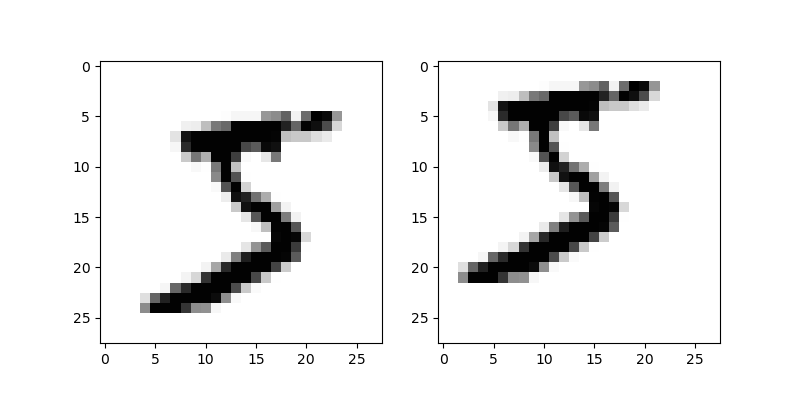
\includegraphics[width=0.5\textwidth]{imgs/img_shift.png}
    \caption{Data augmentation: image shifting}
    \label{fig 1}
\end{figure}

The second approach which is often used in classical machine learning is just adding noise to the data, but this is not a good option for WNN. As for WNN data should be binarised. Thus, effect of adding noise to the initial image will be canceled  after binarisation, resulting in the same binary observation. Therefore we propose the following technique.

After thermometer encoding, we invert certain number of bits. Inverting arbitrary bits may produce unrealistic pictures and may only harm the model (eg. coloring central pixels inside 0 digit). Thus, we propose the following approach. First, we define some probability $p$. Then, every black pixel which has at least one white pixel neighbour can become white with probability $p$. Every white pixel which has at least one black pixel neighbour can become black with probability $p$. As a result, after corrupting the picture, it still remains recognizable. In case of MNIST dataset we still get numbers, only written as if in a different handwriting (see \ref{fig 2}).

\begin{figure}[h]
    \centering
    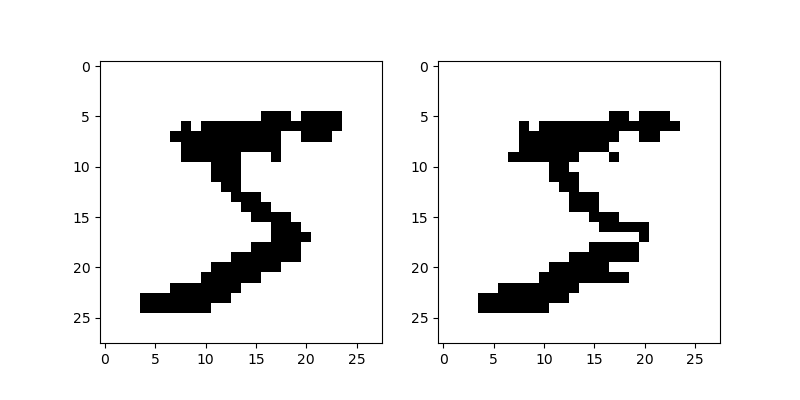
\includegraphics[width=0.5\textwidth]{imgs/img_corruption.png}
    \caption{Data augmentation: image corruption}
    \label{fig 2}
\end{figure}

It is worth mentioning that data augmentation can be especially usefull due to the way WNN learn. Basically, the model just remembers every observation it was given. Thus if during the inference it is given the observation which is just shifted to the left, the model will have troubles of identifying it. General approach to tackle the problem is to randomly split the image into groups of pixels, but anyway it may not produce the desired result - result strongly depends on random partitioning. Thus, data augmentation can reduce randomness by just making training data more versatile.

It is worth mentioning that data augmentation do not affect the size of the model as well as proccessing speed of the model on the inference stage. Training, obviously, takes longer time due to larger amount of training data.

\subsubsection*{Deleting uninformative bits of information}
After binarisation, even when thermometer enconding is used, uninformative bits appear. These bits are the same (or almost the same) for all observations from the dataset (eg. corner pixels are 0 for all pictures). Obviously, such bits do not carry information about whether the observation belongs to certain class. We mark these bits as "bad" and do not use them from now on. Thus, when image is getting split on groups of bits, these "bad" bits are omitted.

\subsubsection*{Reducing dimensionality}
In some cases one may want to reduce dimensionality of the data, for example, when dealing with high resolution images. We are seeking for relatively fast method that effectively reduces size of the observation. Such method is pooling (min, max, avg). Taking into account that data is anyway binarised, the use of this method does not cause significant loss of information (of course when size of the filter is relatively small in comparison with initial image). Moreover, for some pictures we may even benefit from pooling, because pooling reduces fuzziness near color transition boundaries, which is useful for binarization.

\subsection{Feature extraction}
\subsubsection*{Idea}
Features is a built-in ability of any multilayer neural network (eg. feature extractor part which is often used in transfer learning). Our idea was to inherit best practices from standard neural networks and somehow make them applicable to weightless neural networks. Thus, we decided to let model decide by itself which features are good and which are bad. The question remains, how can this be done without the possibility of classical model training? Backpropogation on the one hand is a "superpower" of conventional neural networks, but on the other makes models non-explainable. For the vast majority of models we are not able to understand what and how it learns. However, this is not the case for WNNs. In WNN we can explicitly evaluate each feature learnt and remove if it is useless.

\subsubsection*{Approach to feature extraction}
First of all, we should define what is feature in case of WNN. Of course, one can consider single bit of the data after binarisation as a feature, but single bit on its own, in the vast majority of cases, is not informative. Here and after we define feature a group of bits which is passed to a specific filter. In classical WNN and BTHOWeN\footnote{WNN structure under consideration} observation is splitted on groups of bits manually and each is assigned to specific filter. Thus, we are aware of which filter corresponds to which feature. Evaluating the performance of each filter individually will allow us to assess the significance of each individual feature. Therefore, it remains only to determine what is significance of the feature.

To answer the aforementioned question, we should define what we want from one individual feature. Obviously, it is not correct to demand from a single feature the correct classification of observation. This is a situation when corresponding filter returns \textbf{1} only in the discriminator corresponding to the class of the observation under the study, because one feature can shared among several classes. Both digits "6" and "8" have circle at the bottom, but still "have circle at the bottom" is a very useful feature as it allows model to immediately distinguish these two digits from other classes using the single feature. However, if we consider feature "empty space in the corner of an image", despite the fact that corresponding filter will return \textbf{1} in the discriminator of the correct class, it will also return \textbf{1} in all other discriminators, making this particular feature completely uninformative. To sum up, we desire the filter, corresponding to the property, to always return \textbf{true} for its class, but at the same time there must be at least some classes for which the filter would return \textbf{false}.

To determine the significance of a feature in a strict way, we introduce two criteria. Let's define set of features $\mathcal{F} = \{f_k|k=1,\dots,M\}$ and denote each filter inside a model as $\phi_{j,f_k}$, where $j$ is the number of discriminators (or number of classes) and $f_k$ is a feature corresponding to the given filter. Then, we introduce accuracy of the feature as a ratio of the number of cases when filter, corresponding to the feature in question, returned \textbf{1} in the discriminator corresponding to the class of the considered observation (\ref{acc f}) to number of observations in total.
\begin{equation}\label{acc f}
    acc(f_k) = \frac{\sum_{i=1}^{N}\mathbf{1}_{\phi_{y_i,f_k}(x_i) = 1}(x_i)}{N}
\end{equation}
where $X = \{x_i|i=1,\dots,N\}, Y = \{y_i,i=1,\dots,N\}$ are observations and labels accordingly.
Secondly, we define ordinariness of the feature as a ratio of discriminators for which corresponding filter returned \textbf{1} to the total number of discriminators (number of classes) (\ref{uni f}) averaged over all observations. If $ord(f_k) \approx 1$ this is the case when feature is "empty space in the corner of an image" described above.
\begin{equation}\label{uni f}
    ord(f_k) = \frac{1}{N}\sum_{i=1}^{N}\frac{\sum_{j=1}^{C}\mathbf{1}_{\phi_{j,f_k}(x_i) = 1}(x_i)}{C}
\end{equation}
where $C$ is a number of discriminators (number of classes).

Next, we introduce two hyperparameters $\alpha \in [0,1], \beta \in [0,1]$. So, we call feature to be $\alpha,\beta$ if two conditions are satisfied:
\begin{equation}
    (acc(f_k) \ge \alpha) \wedge (ord(f_k) \le \beta)
\end{equation}
and set of $\alpha\beta$-significant features is denoted as $\mathcal{F}^{\alpha\beta} = \{f_k| (acc(f_k) \ge \alpha) \wedge (ord(f_k) \le \beta)\}$. To select appropriate values of $\alpha, \beta$ either common sense can be used (as this hyperparameters are easy to interpret) or a validation set.

Now when we defined $\alpha\beta$-significance, we can use the following criterion to select features. We propose two ways how feature selection can be applied for WNNs: model reduction and model construction.

\subsubsection*{Model reduction using feature selection}
Model reduction using feature selection based on $\alpha\beta$-significance involves simply deleting filters corresponding to $\alpha\beta$-insignificant features. This approach allows as to reduce size of the model throwing away least important features.

\subsubsection{Model construction using greedy algorithm for feature selection}
The standard approach for choosing features (splitting binarised image on group of pixels) for BTHOWeN model (or other WNN) is a random split. Obviously, such approach does not guarantee that all features will be usefull. To construct model containing important features, we propose the following greedy algorithm:
\begin{enumerate}
    \item Initialise $\mathcal{F}^{\alpha\beta} = \{\}$. Define hyperparameters $\alpha, \beta$ and the number of $\alpha\beta$-significant features to be included $\gamma$.
    \item Generate $\mathcal{F}$ by randomly splitting binarised picture on groups of pixels.
    \item For $f_k$ in $\mathcal{F}$:
    \begin{enumerate}
        \item Fit model with a single feature.
        \item On the validation set find bleach value which guarantees $ord(f_k) \le \beta$ and the same time maximises $acc(f_k)$.
        \item If $acc_{max}f(k) \ge \alpha$ and $f_k$ does not have more than half of the pixels in common with any $f^{\alpha\beta}\in\mathcal{F}^{\alpha\beta}$ (prohibiting  similar features), then we add $f_k$ to set $\mathcal{F}^{\alpha\beta}$ and save its best bleach value.
        \item If $|\mathcal{F}^{\alpha\beta}| = \gamma$ we stop.
    \end{enumerate}
    \item If $|\mathcal{F}^{\alpha\beta}| < \gamma$, go to step 2.
\end{enumerate}
Notice, that the proposed algorithm not only allows to generate set of $\alpha\beta$-significant features, but also proposes approximation for the best bleaching value for each feature. Allowing model to learn more complex patterns.

\subsection{Results}
The proposed methods of data preproccesing and feature selection can be applied in various combinations. The reasonableness and efficacy of using one or another approach should be determined for each task individually. Moreover, efficiency of preprocessing method depends on the model architecture as well. Below, we state few conclusions which were made during simulations:

\subsubsection{Results on data augmentation}
Data augmentation can improve performance of the model, but it requires larger WNN model, due to the fact that WNN learns by remebering certain patterns. Data augmentation generates data with larger number of versatile patterns. Thus, larger model is required to distinguish all the possible patterns, otherwise we run it the problem when hashing function start to map different patterns to same values. Thus, when using data augmentation with small models practitioners should be careful as it can only worsen the performance (see table \ref{table 1}).
\begin{table}[h]
    \centering
    \begin{tabular}{|c|c|}
    \hline
    model & accuracy \\
    \hline
       Small MNIST &  0.924\\
    \hline
       Small MNIST with data augmentation  & 0.913\\
    \hline
       Large MNIST &  0.945\\
    \hline
       Large MNIST with data augmentation  & 0.948\\
    \hline
    \end{tabular}
    \caption{Comparing models on MNIST dataset with and without data augmentation. Small model specifications: bits per input = 2, unit inputs = 28, unit entries = 1024, unit hashes = 2, Large model specifications: bits per input = 6, unit inputs = 49, unit entries = 8192, unit hashes = 4}
    \label{table 1}
\end{table}

However, for tiny models one may find useful to apply pooling. As stated previously, tiny models are not able to learn various different patterns. Pooling decreases size of the observations maintaining important patterns (see table \ref{table 2}). Notice, that for the same models, model which is applied to data with pooling with window $2\times{}2$ has twice less filters, so is twice smaller. As a result, we got a model that is half as small, but its accuracy is only 1\% smaller.
\begin{table}[h]
    \centering
    \begin{tabular}{|c|c|}
    \hline
    model & accuracy \\
    \hline
       Tiny MNIST &  0.887\\
    \hline
       Tiny MNIST, max pooling with window 2 by 2  & .876\\
    \hline
    \end{tabular}
    \caption{Tiny model on MNIST dataset with and without pooling. Tiny model specifications: bits per input = 2, unit inputs = 9, unit entries = 128, unit hashes = 1}
    \label{table 2}
\end{table}

\subsubsection{Results on model reduction using feature selection}
Based on the conducted experiments, we can conclude that proposed method allows to effectively decrease size of the model by deleting filters corresponding to $\alpha\beta$-insignificant features. As shown in the table even for a small model we managed to reduce the model by half (deleting 24 features out of 56), losing only 1.3 percent accuracy.
\begin{table}[h]
    \centering
    \begin{tabular}{|c|c|}
    \hline
    model & accuracy \\
    \hline
       Small MNIST &  0.924\\
    \hline
       Small MNIST with feature selection  & 0.911\\
    \hline
    \end{tabular}
    \caption{Small model on MNIST dataset with and without features selection. Small model specifications: bits per input = 2, unit inputs = 28, unit entries = 1024, unit hashes = 2}
    \label{table 2}
\end{table}

\subsubsection{Results on model construction using feature selection}
The greedy algorithm proposed above is computationally very expensive, which significantly increases the training time of the model. According to the conducted experiments, we conclude that in the majority of cases it is not reasonable to apply this algorithm to simple datasets if model parameters are tuned properly, because it gives very little increase in accuracy. Such that if for MNIST dataset we set \texttt{unit\_entries}\footnote{hyperparameters names are inherited from the article where BTHOWeN model is introduced} greater than 28 (number of bits which is count as one feature), then there is very little chance that any feature will be insignificant. As a result, model constructed by the proposed greedy algorithm shows approximatelly same performance (see table). However, we believe that for larger and more complex datasets the following approach should guarantee better results.


\subsubsection{Combination of approaches} \label{best res}
To obtain model with superior performance, combination of proposed approaches can be used. Below we describe procedure that helped us to obtain better model on MNIST dataset in comparison to the BTHOWeN model of approximately the same size.

\begin{enumerate}
    \item Apply max pooling to the images with a kernel of size $2\times{}2$. 
    \item Apply thermometer encoding with bits per input = 2
    \item Find uninformative bits and denote them as "bad"
    \item Generate features. Instead of generating random features, we use the following approach. We define a sliding window of size $3 \times 3$ and place this windows in each possible position. If no bit is "bad", we add this combination of bits to features.
    \item After this procedure we still get a lot of feature and many of them overlap with each other. Thus we construct model using greedy algorithm for feature selection.
\end{enumerate}

For this approach we defined the following parameters for the model: bits per input = 2, unit inputs = 9, unit entries = 512, unit hashes = 2. Number of features used is 125\footnote{Notice that if we haven't applied data preprocessing and feature selection, then the total number of features for 2 bits per input will be $(28-3+1)^2 = 676$}. Thus, we obtained model approximatelly of the size of the MNIST small model from the article \cite{susskind2022weightless} (MNIST small model has two times larger filter size, but our model has two times more filters), but with 1\% better accuracy. Accuracy for the given model is equal to 0.944.


\newpage
\section{Writeup: Folding WNN}

\section{Writeup: Scaling WNN}
Training WNNs for more complex datasets with observations having many features inevitably leads to a significant increase in the model size and therefore significant increase in inference time \cite{aleksander2009brief}. To deal with this problem we may apply certain techniques which were mentioned previously.

Firstly, we may apply pooling. Pooling significantly reduces size of the data, but some information may be lost due to this operation. Secondly, we may delete unninformative bits. This operation does not delete any information, but not in every dataset such bits exist. Thirdly, we may apply features selection algorithm proposed. Instead of using all the bits from the encoded observations, we may explicitly control number of features we may want to use and sample significant features using proposed greedy algorithm. We have already showed (see section \ref{best res}) how this combination of methods can be used to dramatically decrease size of the model and with fine hyperparameter tuning even improve accuracy.

We tried fitting BTHOWeN model on a CIFAR10 dataset. Even Large MNIST model from the article \cite{susskind2022weightless} result in only 0.43 accuracy. This implies that it is either required to significantly increase the size of the model or try to apply approaches mentioned above or both.


\section{Writeup: Translating DNN into WNN}
Translating DNNs to WWNs is barely possible. Binarisation of weights is not an option, because rounding weights to 0 or 1 for the trained DNN simply results in a completely new DNN. What can theoretically be done, is to somehow extract features from DNN. These features may be used to select features for the WNN. However, we immediately run into an unsolved problem - creation of explainable deep neural network.

There are some approaches on creating intepretable neural networks which involve combining Formal Concept Analysis with neural networks \cite{parakal2022intrinsically, dudyrev2022human, kuznetsov2022pattern}. However, this is a completely new direction in the field of neural networks research. Thus, no satisfying results were obtained.

\section{Writeup: Training WNN}
Conventional training for WNNs is not applicable, as gradient decent can work only with floating numbers and cannot be applied to discrete tasks. Regarding this question we can only suggest only a sketch of a very "brave" and "reckless" idea.

First, we may try to formulate the task of training the WNN model as a problem of discrete optimisation. Secondly, many tasks of discrete optimisation can be reduced to QUBO problem (minimization of a second degree polynomial in which all variables are either 0 or 1). This problem is equivalent to the problem of finding the ground state in the Ising model, only there, instead of the corresponding spin variables, which are either -1 or 1. That is, we need to find a spin configuration that minimizes the Hamiltonian of the Ising model \cite{glover2018logical}. This problem can be reduced to a problem of finding the solution of a systmem of differential equations \cite{goto2019combinatorial, goto2021high}. Thus, we may try to construct transition from a discrete (binary) problem to a contnous problem and then of how classical training algorithms can be used.


\newpage
\bibliographystyle{abbrv}
\bibliography{sample}

\end{document}